\documentclass[12pt]{report}
\usepackage[utf8]{inputenc}
\usepackage[english]{babel}
\usepackage{graphicx}
\usepackage{amssymb}
\usepackage{amsmath}
\usepackage{listings}
\usepackage{tikz}
\usepackage{float}
\PassOptionsToPackage{hyphens}{url}\usepackage{hyperref}
\usepackage[usestackEOL]{stackengine}
\usepackage{minted}

\usetikzlibrary{
    calc,trees,positioning,arrows,chains,shapes.geometric,%
    decorations.pathreplacing,decorations.pathmorphing,shapes,%
    matrix,shapes.symbols
}
\tikzset{
    block/.style={rectangle, rounded corners, minimum height=3em, draw=black, very thick,, text centered ,text width=7.5em},
    big_block/.style={rectangle, rounded corners, minimum height=3em, draw=black, very thick,, text centered ,text width=10em},
    line/.style={->, thick,shorten >=1.5pt},
    decoration={brace},
    tuborg/.style={decorate},
    tubnode/.style={midway, right=2pt},
}

\graphicspath{{images/}}

\title{Engineering a Programming Language}
\author{Èrik Campobadal Forés}

\begin{document}

\begin{titlepage}
    \begin{center}
        \vspace*{1cm}

        {\huge \textbf{\thetitle}}

        \vspace{0.5cm}

        {\Large \thesubtitle}

        \vfill

        {\large \textbf{\textsl{\MakeUppercase{\theauthor}}}}

        \vfill

        \theintro

        \vspace{0.75cm}

        \includegraphics[height=3.5cm]{upc}

        \vspace{0.75cm}

        \themeta

    \end{center}
\end{titlepage}


\tableofcontents
\listoffigures

\chapter{Introduction}
Programming languages are used everyday by thousands of engineers and yet few of them understand how they work.
A programming language is basically the syntax and grammar used as humans to tell a computer what to do. When
somebody wants a computer to do something, it needs to write a program using a programming language and then
a compiler needs to translate it into machine code for the computer to be able to execute it.

To design such a software system, it's vital to understand the theory behind it and learn about all the different
steps involved to make a computer understand and execute a custom programming language.

\section{Objectives}

The objectives of this document are to define and implement a fully featured experimental programming language to learn and
overcome the diferent challenges that are presented during the process. This document also explains and implement
all the different aspects of the programming language ecosystem. This includes for instance the standard library,
dependency management and a full featured webpage for the language. The experimental language is called \textbf{Nuua}.

To better summarize the objectives, this list should give a great overview to understand what this document achieves.

\begin{itemize}
    \item Understand the theory behind all steps involved in common programming languages to be able to reproduce them and adapt it
        at the needs of the project.
    \item Define a non-ambiguous grammar for the Nuua Programming Language. This grammar must be simple, elegan and yet it needs to follow the most
        common programming language's specifications to avoid confusion when learning it, allowing either mature programmers or newcomers to
        pick up the grammar quickly and efficiently.
    \item Choose an efficient programming language to code the language with. The language would need to be efficient, fast and yet able to code with it
        pretty fast to avoid wasting time. Among other options, the languages that satify the previous statement are low level programming languages like
        C, C++, D, Rust, Go, Crystal or Nim.
    \item Define a scalable project structure to allow the programming language to grow efficiently without creating a
        big ball of mud \footnote{\href{https://en.wikipedia.org/wiki/Big_ball_of_mud}{Big ball of mud (Wikipedia)}}. The software system
        that is chosen will be very important towards the scalability of the project.
    \item Create the programming language with a defined set of features found in most programming languages. Those include from basic datatypes
        to object oriented programming.
    \item Create a Standard Library with a common set of operations and also common libraries to work with diferent data types in
        a higher level of abstraction (For example data collections).
    \item Create a cloud centralized dependency manager to allow the programs to require certain libraries with a certain version. Possible
        references are NPM (Node Package Manager), Composer (PHP package manager), Cargo (Rust package manager) or Go mods (Go modules).
    \item Develop the project's website to showcase the language, store the documentation and host the information for the dependency manager.
\end{itemize}

\section{High level overview}

To firstly understand all the complex system that this document implements, it's important to explain a few key concepts
found in a typical compiler. This section details the most important aspects found in a typical programming language and in a compiler infrastructure.
This high level overview won't deal with details and only explains the basics to understand the whole system without deep understanding.
However is good to note that the most import aspecs can be explained further on their respective chapters.


\subsection{Language grammar}

Most programming languages can be expressed using a notation called \textbf{Backus Naur form} or \textbf{BNF} for short. This notation is a form of formal
grammar (Specifically, a context-free grammar) that is used to specify the rules, grammar and alphabet of a language. The BNF form is often used to write
a language specification, so language implementators are able to implement and understand the grammar and rules of a certain language. This
document uses a variant of the BNF notation called \textbf{Extended Backus Naur form} or \textbf{EBNF} for short with a modified syntax to
write the Nuua language specification.

In short, in a formal language there's two diferent types of symbols. Terminals and non-terminals.

\begin{itemize}
    \item \textbf{Terminals}: Symbols that are literals. In a programming language, literal symbols may refer to signs like '+', '*'
        or even numbers or identifiers. Those are often called tokens and it's part of the result of a lexing process.
    \item \textbf{Non-terminals}: Symbols that can be replaced or often reduced based on the grammar rules. It's replacement or reduction
        ends up beeing a terminal symbol.
\end{itemize}

\noindent
The EBNF notation have the following constraints.

\begin{center}
    \texttt{symbol = pattern;}
\end{center}

\noindent
In this code, \textbf{symbol} represents a non-terminal symbol and \textbf{pattern} represents the current non-terminal symbol grammar rule.
In EBNF there are ways to represent diferent situations. This table releates the EBNF syntax symbols that can be used to define rules.

\begin{center}
    \begin{tabular}{ | l | p{10cm} |}
    \hline
    \textbf{Symbol} & \textbf{Definition} \\ \hline
    \texttt{=} & Used to define a rule. \\ \hline
    \texttt{,} & Used to concatenate patterns. \\ \hline
    \texttt{|} & Used to define a union of two sets of patterns. \\ \hline
    \texttt{*} & Used to define an exception. \\ \hline
    \texttt{-} & Used to define a union of two sets of patterns. \\ \hline
    \texttt{[...]} & Used to define an optional pattern. \\ \hline
    \texttt{\{...\}} & Used to define an 0 or many pattern. \\ \hline
    \texttt{(...)} & Used to group a pattern. \\ \hline
    \texttt{"..."} or \texttt{'...'} & Used to define a terminal symbol. \\ \hline
    \texttt{(*...*)} & Used to define a comment. \\ \hline
    \texttt{?...?} & Used to define a special pattern. \\ \hline
    \texttt{;} or \texttt{.} & Used to terminate a given grammar rule. \\ \hline
    \end{tabular}
\end{center}

\noindent
The following example defines a set of symbols to define how an integer may look like, allowing any integer to have an optional symbol prefix followed by
as many digits as needed.\\

\noindent
\texttt{integer\\\tab= ["-" | "+"], digit, \{digit\}\\\tab;}\\
\texttt{digit\\\tab= "0"|"1"|"2"|"3"|"4"|"5"|"6"|"7"|"8"|"9"\\\tab;}\\

\noindent
However, this document will use a modified version of EBNF that deals with common regular expression (regex) patterns.
The special symbols found in this modified version are:

\begin{center}
    \begin{tabular}{ | l | p{10cm} |}
    \hline
    \textbf{Symbol} & \textbf{Definition} \\ \hline
    \texttt{:} & Used to define a rule. \\ \hline
    \texttt{\textit{space}} & Used to concatenate patterns (space separated). \\ \hline
    \texttt{|} & Used to define a union of two sets of patterns. \\ \hline
    \texttt{...+} & Used to define a one or more pattern. \\ \hline
    \texttt{...*} & Used to define a zero or more pattern. \\ \hline
    \texttt{...?} & Used to define an optional pattern. \\ \hline
    \texttt{(...)} & Used to group a pattern. \\ \hline
    \texttt{"..."} or \texttt{'...'} & Used to define a terminal symbol. \\ \hline
    \texttt{;} & Used to terminate a given grammar rule. \\ \hline
    \end{tabular}
\end{center}

\noindent
So the previous example grammar would now be written as:\\

\noindent
\texttt{integer\\\tab: ("-" | "+")? digit+\\\tab;}\\
\texttt{digit\\\tab: "0"|"1"|"2"|"3"|"4"|"5"|"6"|"7"|"8"|"9"\\\tab;}\\

\noindent
This variation is often used by many parser generators since it introduces a more visible and versatile aproach to
write the language grammar.

\subsection{Compilers}

The job of a compiler is to take an input source and translate it into another. Often, the compiler term is used to express
a translation to a much diferent environment, that means that usually, the input is written in a high level language and further
translated into a lower level of abstraction. As an example, GCC (GNU Compiler Collection) and it's implementation of the C programming
language basically compiles the input code into assembly (and optimized if needed), then to an object file and finally linked
to generate an executable. That said, the compiler job was to translate a high level programming language (C) into a low level programming
language (Assembly). However, there are multiple types of compilers, and each one is used to implement different translation tasks.

\begin{itemize}
    \item \textbf{Compiler}: Translates a high level language to a low level language in the same or diferent architecture.
        For example, GCC's C implementation
    \item \textbf{Cross-Compiler}: The translation is done to a specific (and probably diferent than the compiler's machine) architecture.
        For example, AVR-GCC compiles specifically for the AVR microcontroller architecture. Other closer examples may be found when compiling for
        32 bits or 64 bits target architecture.
    \item \textbf{Bootstrap compiler}: A compiler that is built using the language it compiles to (The initial version is written in another language)
        For example, the official Go compiler is written in Go.
    \item \textbf{Decompiler}: Translates a low level language to a high level language in the same or diferent architecture.
        For example, the Boomerang decompiler.
    \item \textbf{Transpiler (Source-to-source compiler)}: Translates a language to a similar level of abstraction (usually between high level languages).
        For example, TypeScript (compiles to JavaScript).
\end{itemize}

\begin{figure}[H]
    \centering
    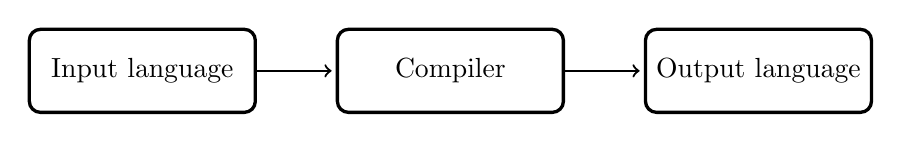
\begin{tikzpicture}
        [node distance=1cm]

        % Nodes of the layered system
        \node[block] (input) {Input language};
        \node[block,right=of input] (compiler) {Compiler};
        \node[block,right=of compiler] (output) {Output language};

        % Lines
        \draw[line] (input) -- (compiler);
        \draw[line] (compiler) -- (output);

    \end{tikzpicture}

    % Caption and Label
    \caption{Compiler overview}
    \label{fig:compiler_overview}
\end{figure}

A compiler job is just to translate, and then, it's up to the language implementation to run it. There are diferent ways to
run or execute a programming language.

\begin{itemize}
    \item \textbf{Machine-language compiler}: Compilers whose target language is executable code (machine-language) can be run
        by the operating system. Machine code have a big advantage and disadvantage. The executed code will be very fast but the
        executable is not portable among diferent architectured. This introduces platform-dependent builds that are very fast.
    \item \textbf{Interpreter}: Interpreters are often a very diferent overview of this problem. Interpreters do not compile
        to machine language and instead it often compiles to bytecode, a portable and reduced instruction set similar to machine instructions
        that is used to execute the language. The advantages are that is platform-independent and it's designed specifically with the language
        needs but one big disadvantage is that it's much slower to run than real machine-code. Interpreters can also make language execution
        dynamic allowing untyped languages that plays around with diferent variable types.
    \item \textbf{Just-in-time compiler}: Just-in-time compilers (often called JIT compilers) are an intermidiate aproach between the other two
        that tries to speed up the execution of interpreters by compiling chunks of code at a specific moment while the program run to speed up portions
        of the code that is often executed (for example functions that are called frequently). Esentially, the JIT compiler needs to decide when to compile
        a specific part of the code at runtime and adds a small overhead in exchange for a machine-language performance on successive calls.
\end{itemize}

\subsection{Phases of a compiler}

A compiler can also be decoupled into diferent parts. Each part does a very different job but they are all connected to each other.
In a typical compiler architecture, we may find all the different phases described in \autoref{fig:compiler_phases}.

Those phases are often found to be diferent depending on the implementation of the language. However, it's important to note what they do,
since they are often implemented in one way or another. More implementation details are explained in their respective chapters but in this
section a small introduction to each phase is needed to understand the Nuua's system.

\begin{figure}[p]
    \centering
    \begin{tikzpicture}
        [node distance=1cm]

        \node (input) {Input};
        \node[bigger_block,below=of input] (lexical) {Lexical analysis (Lexer or scanner)};
        \node[bigger_block,below=of lexical] (syntax) {Syntax analysis (Parser)};
        \node[bigger_block,below=of syntax] (semantic) {Semantic analysis};
        \node[bigger_block,below=of semantic] (inter) {Intermediate code};
        \node[bigger_block,below=of inter] (opt) {Optimization};
        \node[bigger_block,below=of opt] (codegen) {Code generation};
        \node[below=of codegen] (output) {Output};

        \draw[line] (input) -- (lexical);
        \draw[line] (lexical) -- (syntax);
        \draw[line] (syntax) -- (semantic);
        \draw[line] (semantic) -- (inter);
        \draw[line] (inter) -- (opt);
        \draw[line] (opt) -- (codegen);
        \draw[line] (codegen) -- (output);

        % The right specifiers
        \draw[tuborg, decoration={brace}] let \p1=(lexical.north), \p2=(semantic.south) in
            ($(3.5, \y1)$) -- ($(3.5, \y2)$) node[tubnode] {Front end};
        \draw[tuborg, decoration={brace}] let \p1=(inter.north), \p2=(opt.south) in
            ($(3.5, \y1)$) -- ($(3.5, \y2)$) node[tubnode] {Middle end};
        \draw[tuborg, decoration={brace}] let \p1=(codegen.north), \p2=(codegen.south) in
            ($(3.5, \y1)$) -- ($(3.5, \y2)$) node[tubnode] {Back end};
    \end{tikzpicture}

    % Caption and Label
    \caption{Common compiler phases}
    \label{fig:compiler_phases}
\end{figure}

\begin{itemize}
    \item \textbf{Lexical analysis}: In this pahase, the input source is transformed from a character string into a token list, this is also called
        tokenization. Tokens are known and have certain attributes. For example, some tokens might include integers, symbols (+, -, *, etc.) or
        identifiers among others. Lexemes are also evalued as individual tokens, making a single token for identifiers matched as language keywords
        (like 'if', 'while', etc.). This phase is also called lexer or scanner.
    \item \textbf{Syntax analysis}: In this phase, the implementation may vary among compilers, some of them work close to the lexical analysis since they
        can work together. However, its purpose is to perform operations to the token list to parse the input and create an Abstract Syntax Tree
        (AST\footnote{\href{https://en.wikipedia.org/wiki/Abstract_syntax_tree}{Abstract Syntax Tree (Wikipedia)}}). An AST is already a structural representation
        that represents your input source. This stage determines if it is a valid program based on the language grammar and the specified rules. There are also
        scannerless parsers that takes the lexical analysis and the syntax analysis into a single step. It is harder to understand and build but it often leads to
        faster parsing and less memory usage.
    \item \textbf{Semantic analysis}: This phase analyzes the AST and creates a symbol table while analyzes the input source with things like type checking or
        variable declarations, if some operations can be performed (for example adding a number with a string). A symbol table is a structure used by further
        phases to see information attached to specific source code parts. For example, it can store information about a variable (if it's global, exported, etc.).
    \item \textbf{Intermidiate code}: An intermidiate representation (IR) can be avoided but it's often used to have a platform independent optimizer. Usually
        the code generation target a specific architecture and would require diferent optimizers depending on each architecture. However, by having a IR it's possible
        to have a single optimizer. A much used IR is Three Adress Code (TAC\footnote{\href{https://en.wikipedia.org/wiki/Three-address_code}{Three Address Code (Wikipedia)}})
        that can be organized in quadruples or triples.
    \item \textbf{Optimization}: This optimization is often performed on the IR and performs diferent tasks to allow a faster and smaller output. For example, it may
        remove dead code, perform loop optimizations, etc.
    \item \textbf{Code generation}: This is where the real translation takes place, it translates the IR into a diferent language output. For example machine code.
        This phase often have to deal with instruction scheduling or register allocation while they have to output a fully working program.
\end{itemize}

\section{System architecture}

To design the system architecture of Nuua, a consideration of existing system architectures needs to be taken since existing architectures
often work better than the custom-made ones and they often lead to a greater project scalability. It's trivial
to make this choice before starting the project since changing a system architecture after it's initial
development phases becomes a very bad choice and may lead to a big ball of mud. Two choices in software development might be hierarchical
or layered systems. Nuua's architecture is based on a \textbf{layered system}.\\

\noindent
A layered system have specific constraints regarding to the whole communication. Specifically, a layered system consists
of diferent layers arrenged vertically. Those layers have a specific criteria that needs to be met. As a matter of fact,
each layer can only use the layer below and and gives an API for the layer above (if any) to use it's functions. For example,
the \autoref{fig:layered_system} contains a simple 3-tier layered system. The Layer 3 can only use Layer 2, and the output comes
from Layer 2. Layer 3 can not use Layer 1 nor expect any outputs from it. It's the Layer 2 responsibility to use the Layer 1
and process its output before it can give its own output.

\begin{figure}[H]
    \centering
    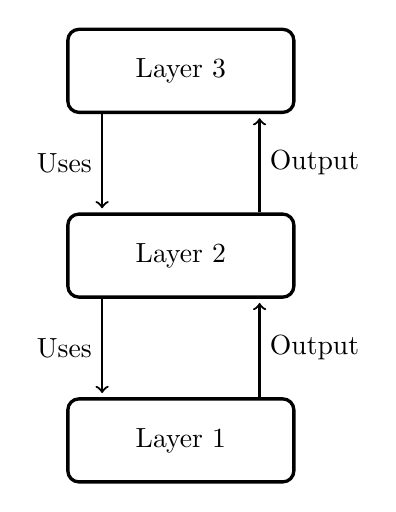
\begin{tikzpicture}
        [node distance=1.25cm]

        % Nodes of the layered system
        \node[block] (layerc) {Layer 3};
        \node[block,below=of layerc] (layerb) {Layer 2};
        \node[block,below=of layerb] (layera) {Layer 1};

        % Arrows going down
        \draw[line] ($(layerc.south) + (-1, 0)$) -- node[midway, left] {Uses} ($(layerb.north) + (-1, 0)$);
        \draw[line] ($(layerb.south) + (-1, 0)$) -- node[midway, left] {Uses} ($(layera.north) + (-1, 0)$);

        % Arrows going up
        \draw[line] ($(layerb.north) + (1, 0)$) -- node[midway, right] {Output} ($(layerc.south) + (1, 0)$);
        \draw[line] ($(layera.north) + (1, 0)$) -- node[midway, right] {Output} ($(layerb.south) + (1, 0)$);

    \end{tikzpicture}

    % Caption and Label
    \caption{Layered system}
    \label{fig:layered_system}
\end{figure}

This system is known to be robust and scalable at very low performance cost. It's very easy to understand and yet very powerful
for software systems like this one. This systems are also used for other complex software systems, such as operating
systems or complex protocols like TCP/IP.\\

\noindent
By using a layered system each layer gets completly isolated and works independently by just using the layer below,
creating a very impresive way to scale-up or upgrade existing parts of the system without damaging the others.
However, a consistent API should in fact be established from the ground up to avoid breaking changes.
If the API is maintained, the individual layers may be upgraded independently without the need of extra work.\\

\noindent
The Nuua architecture is shown at \autoref{fig:nuua_system}. An independent module called Logger is found
on the left side of the figure. This module is a logger used by all layers to output messages if needed (for example error reporting).

\begin{figure}[p]
    \centering
    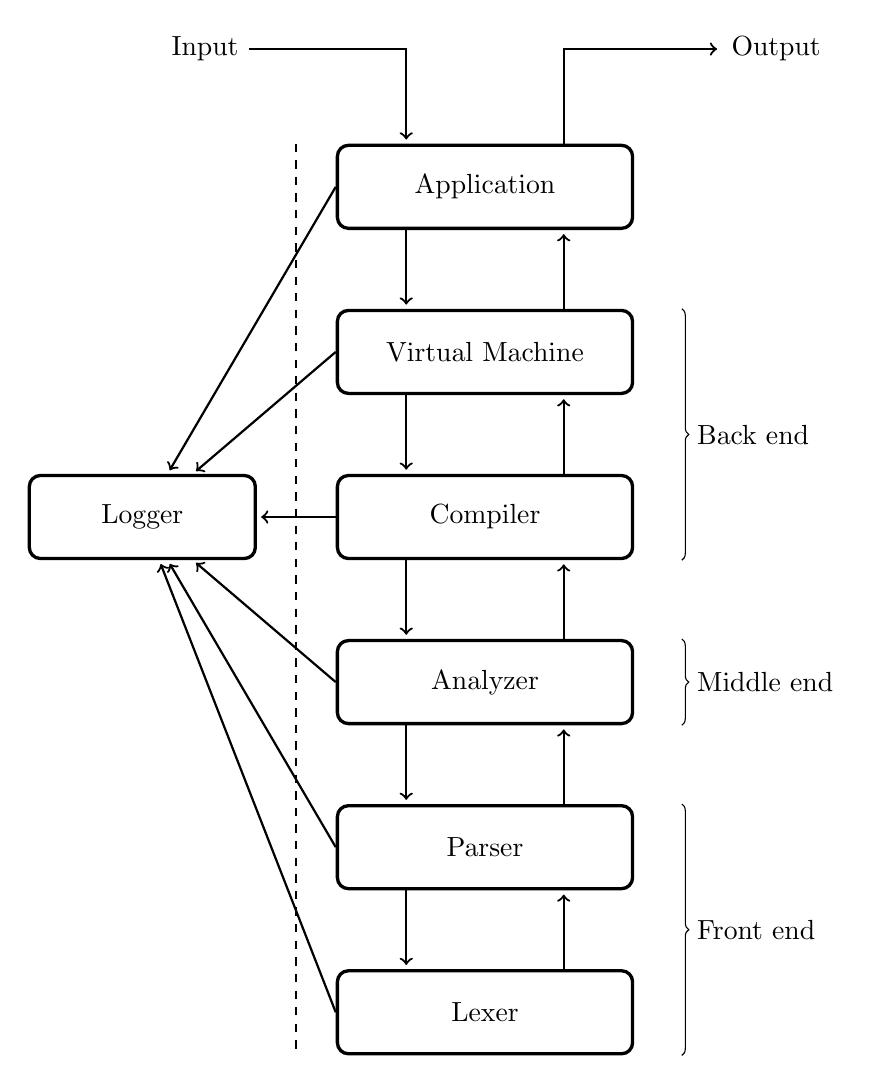
\begin{tikzpicture}
        [node distance=1cm]

        % Nodes of the layered system
        \node[big_block] (app) {Application};
        \node[big_block,below=of app] (vm) {Virtual Machine};
        \node[big_block,below=of vm] (compiler) {Compiler};
        \node[big_block,below=of compiler] (analyzer) {Analyzer};
        \node[big_block,below=of analyzer] (parser) {Parser};
        \node[big_block,below=of parser] (lexer) {Lexer};

        % Independent module
        \node[block, left=of compiler] (logger) {Logger};

        % Separator
        \draw[thick,dashed] ($(app.north west) + (-0.5, 0)$) -- ($(lexer.south west) + (-0.5, 0)$);

        % Top arrows
        \draw[line] (-3, 1.75) node[anchor=east] {Input} -| ($(app.north) + (-1, 0)$);
        \draw[line] ($(app.north) + (1, 0)$) |- (3, 1.75) node[anchor=west] {Output};

        % Arrows going down
        \draw[line] ($(app.south) + (-1, 0)$) -- ($(vm.north) + (-1, 0)$);
        \draw[line] ($(vm.south) + (-1, 0)$) -- ($(compiler.north) + (-1, 0)$);
        \draw[line] ($(compiler.south) + (-1, 0)$) -- ($(analyzer.north) + (-1, 0)$);
        \draw[line] ($(analyzer.south) + (-1, 0)$) -- ($(parser.north) + (-1, 0)$);
        \draw[line] ($(parser.south) + (-1, 0)$) -- ($(lexer.north) + (-1, 0)$);

        % Arrows going up
        \draw[line] ($(vm.north) + (1, 0)$) -- ($(app.south) + (1, 0)$);
        \draw[line] ($(compiler.north) + (1, 0)$) -- ($(vm.south) + (1, 0)$);
        \draw[line] ($(analyzer.north) + (1, 0)$) -- ($(compiler.south) + (1, 0)$);
        \draw[line] ($(parser.north) + (1, 0)$) -- ($(analyzer.south) + (1, 0)$);
        \draw[line] ($(lexer.north) + (1, 0)$) -- ($(parser.south) + (1, 0)$);

        % Logger arrows
        \draw[line] (app.west) -- (logger);
        \draw[line] (vm.west) -- (logger);
        \draw[line] (compiler.west) -- (logger);
        \draw[line] (analyzer.west) -- (logger);
        \draw[line] (parser.west) -- (logger);
        \draw[line] (lexer.west) -- (logger);

        % The right specifiers
        \draw[tuborg, decoration={brace}] let \p1=(parser.north), \p2=(lexer.south) in
            ($(2.5, \y1)$) -- ($(2.5, \y2)$) node[tubnode] {Front end};
        \draw[tuborg, decoration={brace}] let \p1=(analyzer.north), \p2=(analyzer.south) in
            ($(2.5, \y1)$) -- ($(2.5, \y2)$) node[tubnode] {Middle end};
        \draw[tuborg, decoration={brace}] let \p1=(vm.north), \p2=(compiler.south) in
            ($(2.5, \y1)$) -- ($(2.5, \y2)$) node[tubnode] {Back end};
    \end{tikzpicture}

    % Caption and Label
    \caption{Nuua's architecture (Layered System)}
    \label{fig:nuua_system}
\end{figure}

\begin{itemize}
    \item \textbf{Logger}: Used by all layers to debug or log errors. In case of a fatal error, the logger outputs
        an error stack in a fancy way and terminates the application.
    \item \textbf{Application}: This layer is used to decode the command line arguments and fire up the compiler toolchain. In short, it's
        purpose is to analyze the command line arguments and fire the application acordingly.
    \item \textbf{Virtual Machine}: The virtual machine is the interpreter that runs Nuua. It's a register-based virtual machine that
        acts as the nuua runtime environment.
    \item \textbf{Compiler}: Is responsible of the translation of the AST to the virtual machine bytecode. This acts as the code generation
        part of a compiler architecture.
    \item \textbf{Analyzer}: Does all the semantic analysis of the compiler and optimizes the AST for a faster and smaller output.
    \item \textbf{Parser}: Acts as the syntax analyzer, it uses a list of tokens and generates a fully valid AST.
    \item \textbf{Lexer}: Scans the source code and translates the characters to a tokens, creating a list of tokens representing
        the original source code.
\end{itemize}


\chapter{The Nuua Language}
This chapter defines the Nuua programming language. The language is set to be of a general purpose usage, with an inperative
paradigm and a statically typed system. The official Nuua compiler is written in C++ with a zero-dependency policy and it's
implemented as an interpreter using a register-based virtual machine.

\section{Nuua Grammar}

Nuua's grammar is inspired by other existing programming languages by taking advantage of some of the best features some of them offer.
Inspiration comes specially from Python, Rust and Go.

The precedence relationship between expressions is heavily inspired by C, D, Rust and Dart. The official documentation for those languages
exposes similar tables for operator precedences and Nuua has taken akin levels of precedence as those.

Nuua does not make use of the \texttt{';'} to separate statements, instead, it uses the same separator as Go. Statements can be separated by
a \texttt{'\textbackslash n'} but it does not make use of the \texttt{\textbackslash t} to indicate statements inside blocks, and uses the typical
block separator \texttt{\{ ... \}}.

\subsection{Lexical Grammar}

The lexical grammar is used by the lowest layer of the Nuua system to scan the source language and identify different terminal symbols.
The main difference with the syntax grammar, as exposed in \autocite[Appendix~I]{crafting_interpreters} is that the syntax grammar is a
context free grammar and the lexical grammar is a regular grammar.

Nuua's lexical rules are as follors:

\texttt{
    DIGIT\\
        \tab: '0' ... '9'\\
        \tab;
}

Digits are any character from '0' to '9', given that the ASCII table \footnote{\href{https://en.wikipedia.org/wiki/ASCII}{ASCII table (Wikipedia)}} uses
a sequential enumeration for them, it's very easy to determine what characters are between '0' and '9'.

\texttt{
    ALPHA\\
        \tab: 'a' ... 'z'\\
        \tab| 'A' ... 'Z'\\
        \tab| '\_'\\
        \tab;
}

Alpha are characters that are part of the english alphabet in lower or upper case. It also includes '\_' as a special character.

\texttt{
    ALPHANUM\\
        \tab: DIGIT\\
        \tab| ALPHA\\
        \tab;
}

Alphanum are characters that are either part of the alphabet or are digits.

\texttt{
    INTEGER\\
        \tab: DIGIT+\\
        \tab;
}

Integers are a single digit or more found sequentially without spaces. The integer sign is not represented here.

\texttt{
    FLOAT\\
        \tab: DIGIT+ '.' DIGIT+\\
        \tab;
}

Floats are like integers but require a dot followed by a digit or more, creating a decimal number.

\texttt{
    BOOL\\
        \tab: 'true'\\
        \tab| 'false'\\
        \tab;
}

Bools are either 'true' or 'false', that are reserved words.

\texttt{
    STRING\\
        \tab: '"' \# '"' \# '"'\\
        \tab;
}

Strings represent a character string with the possibility to escape '"' by using a '\textbackslash' as a prefix, more on that in the upcomming sections.

\texttt{
    IDENTIFIER\\
        \tab: ALPHA ALPHANUM*\\
        \tab;
}

Identifiers are part an alpha character followed by an optional one or more alphanumeric character.

\subsection{Syntax Grammar}

\subsubsection{Program and Top Level Declarations}

\texttt{
    program\\
        \tab: top\_level\_declaration*\\
        \tab;
}

A Nuua program is a list of top level declarations.

\texttt{
    top\_level\_declaration\\
        \tab: use\_declaration '\textbackslash n'\\
        \tab| export\_declaration '\textbackslash n'\\
        \tab| class\_declaration '\textbackslash n'\\
        \tab| fun\_declaration '\textbackslash n'\\
        \tab;
}

A top level delcaration can only be one of the specified rules. Top level declarations are a
special type of declaration that can only be declared on the module and not inside other blocks.

\texttt{
    export\_declaration\\
        \tab: "export" top\_level\_declaration\\
        \tab;
}

An export declaration marks the following top level declaration as exported, making it available for other modules to import it using the
use declaration.

\texttt{
    use\_declaration\\
        \tab: "use" STRING\\
        \tab| "use" IDENTIFIER ("," IDENTIFIER)* "from" STRING\\
        \tab;
}

A use declaration is used to import other top level declarations from other modules. By using the first rule, Nuua imports all the
exported targets of the module pointed by STRING. Otherwise, Nuua imports the specified targets from the modules.

\texttt{
    class\_declaration\\
        \tab: "use" STRING\\
        \tab| "use" IDENTIFIER ("," IDENTIFIER)* "from" STRING\\
        \tab;
}

\subsubsection{Expressions}

\texttt{
    LIST\\
        \tab: "[" expression (',' expression)* "]"\\
        \tab;
}

Lists can't be empty, so a at least one expression must be provided.

\texttt{
    DICTIONARY\\
        \tab: "\{" IDENTIFIER ':' expression (',' IDENTIFIER ':' expression)* "\}"\\
        \tab;
}

Dictionaries, as lists, can't be empty, so a at least one expression must be provided.

\subsection{Operator precedence}


\end{document}
